\documentclass[onecolumn, draftclsnofoot,10pt, compsoc]{IEEEtran}
\usepackage{graphicx}
\usepackage{setspace}
\usepackage{comment}
\usepackage{bigstrut}
\usepackage{geometry}
\usepackage{supertabular}

\usepackage{fancyhdr}
\usepackage{csquotes}

\usepackage{tabu}
\usepackage{hyperref}
\usepackage{url}
\hypersetup{
	colorlinks=true, linkcolor=blue, citecolor=blue, filecolor=blue, urlcolor=blue}
\geometry{textheight=9.5in, textwidth=7in}

\usepackage{color}
\definecolor{editorGray}{rgb}{0.95, 0.95, 0.95}
\definecolor{editorOcher}{rgb}{1, 0.5, 0} % #FF7F00 -> rgb(239, 169, 0)
\definecolor{editorGreen}{rgb}{0, 0.67, 0} % #007C00 -> rgb(0, 124, 0)

\usepackage{listings}
\lstdefinelanguage{JavaScript}{
	morekeywords={typeof, new, true, false, catch, function, return, null, catch, switch,
		var, if, in, while, do, else, case, break, addChapter, await},
	morecomment=[s]{/*}{*/},
	morecomment=[l]//,
	morestring=[b]",
	morestring=[b]'
}
\usepackage{color}
\definecolor{editorGray}{rgb}{0.95, 0.95, 0.95}
\definecolor{editorOcher}{rgb}{1, 0.5, 0} % #FF7F00 -> rgb(239, 169, 0)
\definecolor{editorGreen}{rgb}{0, 0.67, 0} % #007C00 -> rgb(0, 124, 0)

\usepackage{listings}
\lstdefinelanguage{JavaScript}{
	morekeywords={typeof, new, true, false, catch, function, return, null, catch, switch,
		var, if, in, while, do, else, case, break, addChapter, await},
	morecomment=[s]{/*}{*/},
	morecomment=[l]//,
	morestring=[b]",
	morestring=[b]'
}

\lstset{%
	% Basic design
	backgroundcolor=\color{editorGray},
	basicstyle={\small\ttfamily},
	frame=l,
	% Line numbers
	xleftmargin={0.75cm},
	numbers=left,
	stepnumber=5,
	firstnumber=1,
	numberfirstline=true,
	% Code design
	keywordstyle=\color{blue}\bfseries,
	commentstyle=\color{red}\ttfamily,
	ndkeywordstyle=\color{editorOcher}\bfseries,
	stringstyle=\color{editorGreen},
	% Code
	language=JavaScript,
	alsodigit={.:;},
	tabsize=2,
	showtabs=false,
	showspaces=false,
	showstringspaces=true,
	extendedchars=true,
	breaklines=true
}

\pagestyle{fancy}
\fancyfoot[C]{APPENDIX --- \thepage}
\setlength\parindent{0pt}

\begin{document}
	
	\section{Code Examples}
	\noindent The backend is split into two primary parts. The first, and most difficult part
	of the backend, is the interface library being used to store objects into the
	git repositories and to get them back out. Shown below is a code sample, which
	is fully working today, showing a simple script that creates new scraps,
	chapters, and books, and gets a valid latex document to render from them. 
	Below are two interesting pieces of backend code that allow the user to have 
	a seamless experience combining different scraps, chapters, and books together.
	
	\begin{lstlisting}
	var a = new scrap.Scrap('First sentence of a chapter', 'rambourg');
	await a.save('initial save');
	
	var b = new scrap.Scrap('Second sentence of a chapter', 'rambourg');
	await b.save('initial save');
	
	var ch1 = new chapter.Chapter('First Chapter Name', 'rambourg');
	ch1.addScrap(a);
	ch1.addScrap(b);
	
	await ch1.save('initial save');
	
	var c = new scrap.Scrap('First sentence of another chapter', 'rambourg');
	await c.save('initial save');
	var ch2 = new chapter.Chapter('Another Chapter Title', 'rambourg');
	ch2.addScrap(c);
	await ch2.save('initial save');
	
	var myBook = new Book('My Fav Book Title', 'rambourg');
	myBook.addChapter(ch1);
	myBook.addChapter(ch2);
	
	var bookText = await myBook.getText();
	\end{lstlisting}
	
	\newpage
	\noindent Another piece of interesting code that we want to highlight is the creation of a new scrap. In the code example below, we determine whether this new scrap is going to be appended to an existing chapter, and if so, we need to first return and collect all of the existing scraps associated with that chapter. Once we have the new list of scraps, we need to update the chapter object with the new information.

	\begin{lstlisting}
	var scr = new scrap.Scrap('Brody', 'abc123-def456')
	
	/* reconstitute a chapter from author and id */
	var ch = chapter.reconstitute('Patrick Rambourg', '56c2c2ee')
	var newCh = await ch.fork('Brody')
	
	newCh.addScrap(scr)
	await newCh.save('add new chapter')

	submitNewScrap() {
	
	if (this.selectedFile) {
	this.submitImageScrap();
	return;
	}
	
	var requested = this.userText;
	var enableLatex = this.enableLatex;
	var theAuthor = Cookies.get('username');
	var theChapter = this.chapters[1];
	var authToken = "Token " + Cookies.get('token');
	
	var submitTags = this.submitTags;
	var submittedTags = this.submitTagsText;
	
	if (theChapter === undefined || theChapter === null || theChapter === "") {
	if (submitTags) {
	submittedTags = submittedTags.toString();
	submittedTags = submittedTags.replace(/(^,)|(,$)/g, "");
	submittedTags = submittedTags.replace(/\s/g, '');
	submittedTags = submittedTags.split(",");
	}
	let request = {
	author: theAuthor,
	text: requested,
	latex: enableLatex,
	tags: submittedTags
	};
	\end{lstlisting}
	
	
	\newpage
	
	The next code listing to be shown is the new scrap creation process. This is a particularly interesting section of code because it determines what to do for the user. Based on what page the user's request originated the new scrap function will either simply create the scrap and place it within the user's MyScrap page. If the user's request originated from the edit chapter page, it will dynamically build the list of all existing scraps and their ordering, and then append the new scrap and submit the new list to the database.
	
	\begin{lstlisting}
	//CREATE THE NEW SCRAP AND GET THE NEW SCRAP ID
	var scrapID = '';
	httpClient.fetch('https://remix.ist/scraps/new', {
	method: 'post',
	body: JSON.stringify(request),
	headers: {
	'Content-Type': 'application/json',
	'Authorization': authToken
	}
	})
	.then(response => response.json())
	.then(data => {
	var scrapID = data.uuid;
	this.toast.show('Scrap saved successfully!', 5000);
	this.ea.publish('new-scrap', data);
	});
	} else { //The Chapter Was Provided, so create the scrap and then add it to a chapter.
	if (submitTags) {
	submittedTags = submittedTags.toString();
	submittedTags = submittedTags.replace(/(^,)|(,$)/g, "");
	submittedTags = submittedTags.replace(/\s/g, '');
	submittedTags = submittedTags.split(",");
	}
	
	let request = {
	author: theAuthor,
	text: requested,
	latex: enableLatex,
	tags: submittedTags
	};
	
	//CREATE THE NEW SCRAP AND GET THE NEW SCRAP ID
	var scrapID = '';
	httpClient.fetch('https://remix.ist/scraps/new', {
	method: 'post',
	body: JSON.stringify(request),
	headers: {
	'Content-Type': 'application/json',
	'Authorization': authToken
	}
	})
	.then(response => response.json())
	.then(data => {
	var new_scrap = data;
	var scrapID = data.uuid;
	
	this.scraps = [];
	var test = [];
	//GET CHAPTERS SCRAPS
	httpClient.fetch('https://remix.ist/chapters/' + theAuthor + '/' + theChapter)
	.then(response => response.json())
	.then(data => {
	
	var scraps;
	this.scraps.push(data);
	scraps = data.scraps;
	
	var newScrapRequest = [];
	
	for (var i = 0; i < scraps.length; i++) {
	newScrapRequest.push([scraps[i][0], scraps[i][1], scraps[i][2]]);
	}
	newScrapRequest.push([theAuthor, scrapID, null]);
	let request2 = {
	scraps: newScrapRequest
	};
	
	//   UPDATE CHAPTER WITH NEW SCRAPS
	httpClient.fetch('https://remix.ist/chapters/' + theAuthor + '/' + theChapter, {
	method: 'post',
	body: JSON.stringify(request2),
	headers: {
	'Content-Type': 'application/json',
	'Authorization': authToken
	}
	})
	.then(response => response.json())
	.then(data => {
	this.toast.show('Scrap saved successfully!', 5000);
	this.ea.publish('new-scrap', new_scrap);
	});
	}
	}
	\end{lstlisting}
	
	\newpage
	\section{Project Images}
	
	\noindent This section is dedicated to showing some of the progress that has been made through iteration and user feedback. Starting with our low level prototypes, medium fidelity prototypes, high fidelity prototypes, and finally our finished product. The designs were influenced by user feedback throughout the development process.
	
	\begin{figure}[ht!]
		\centering
		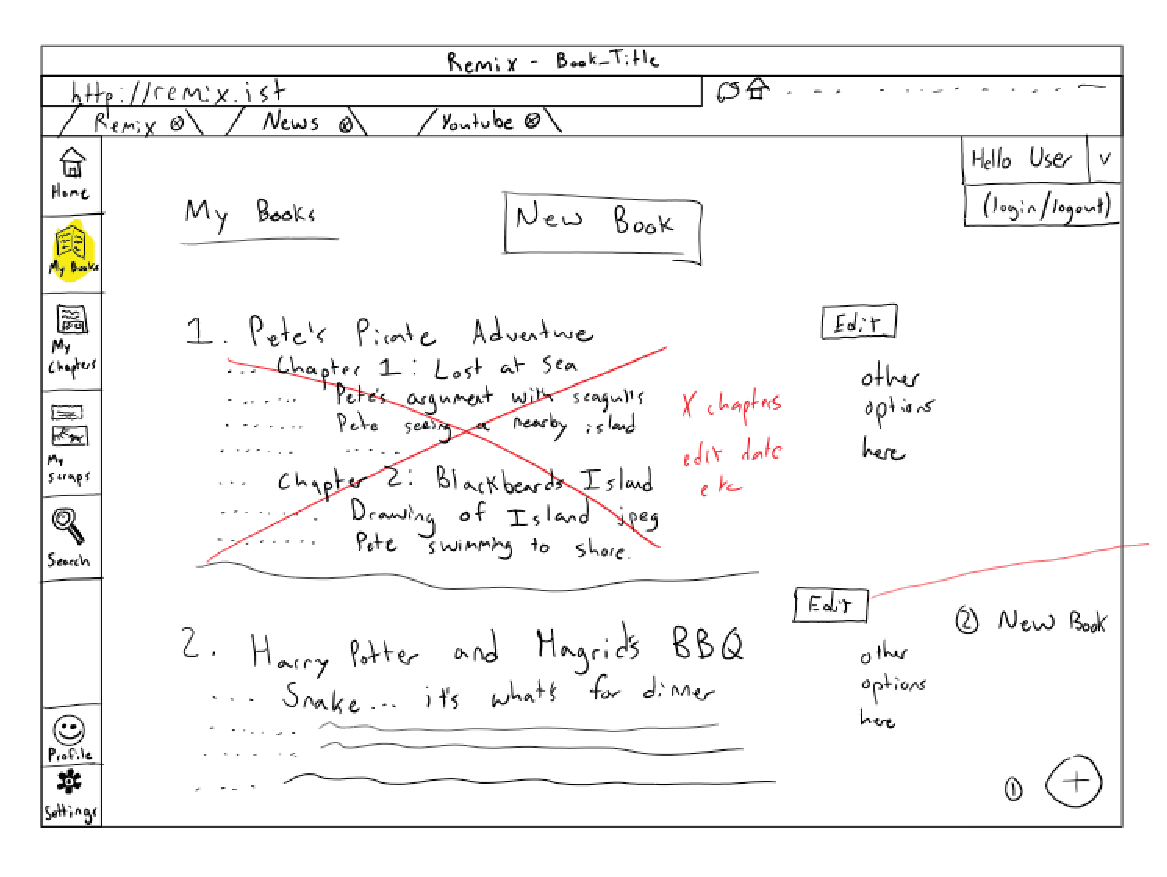
\includegraphics[width=\textwidth]{images/prototype}
		\caption{Here is one low fidelity prototype that was shown to our client. Dr. Jensen suggested 
			removing the preview of chapters and scraps to make the interface a little more simple.}
	\end{figure}
	
	\begin{figure}[ht!]
		\centering
		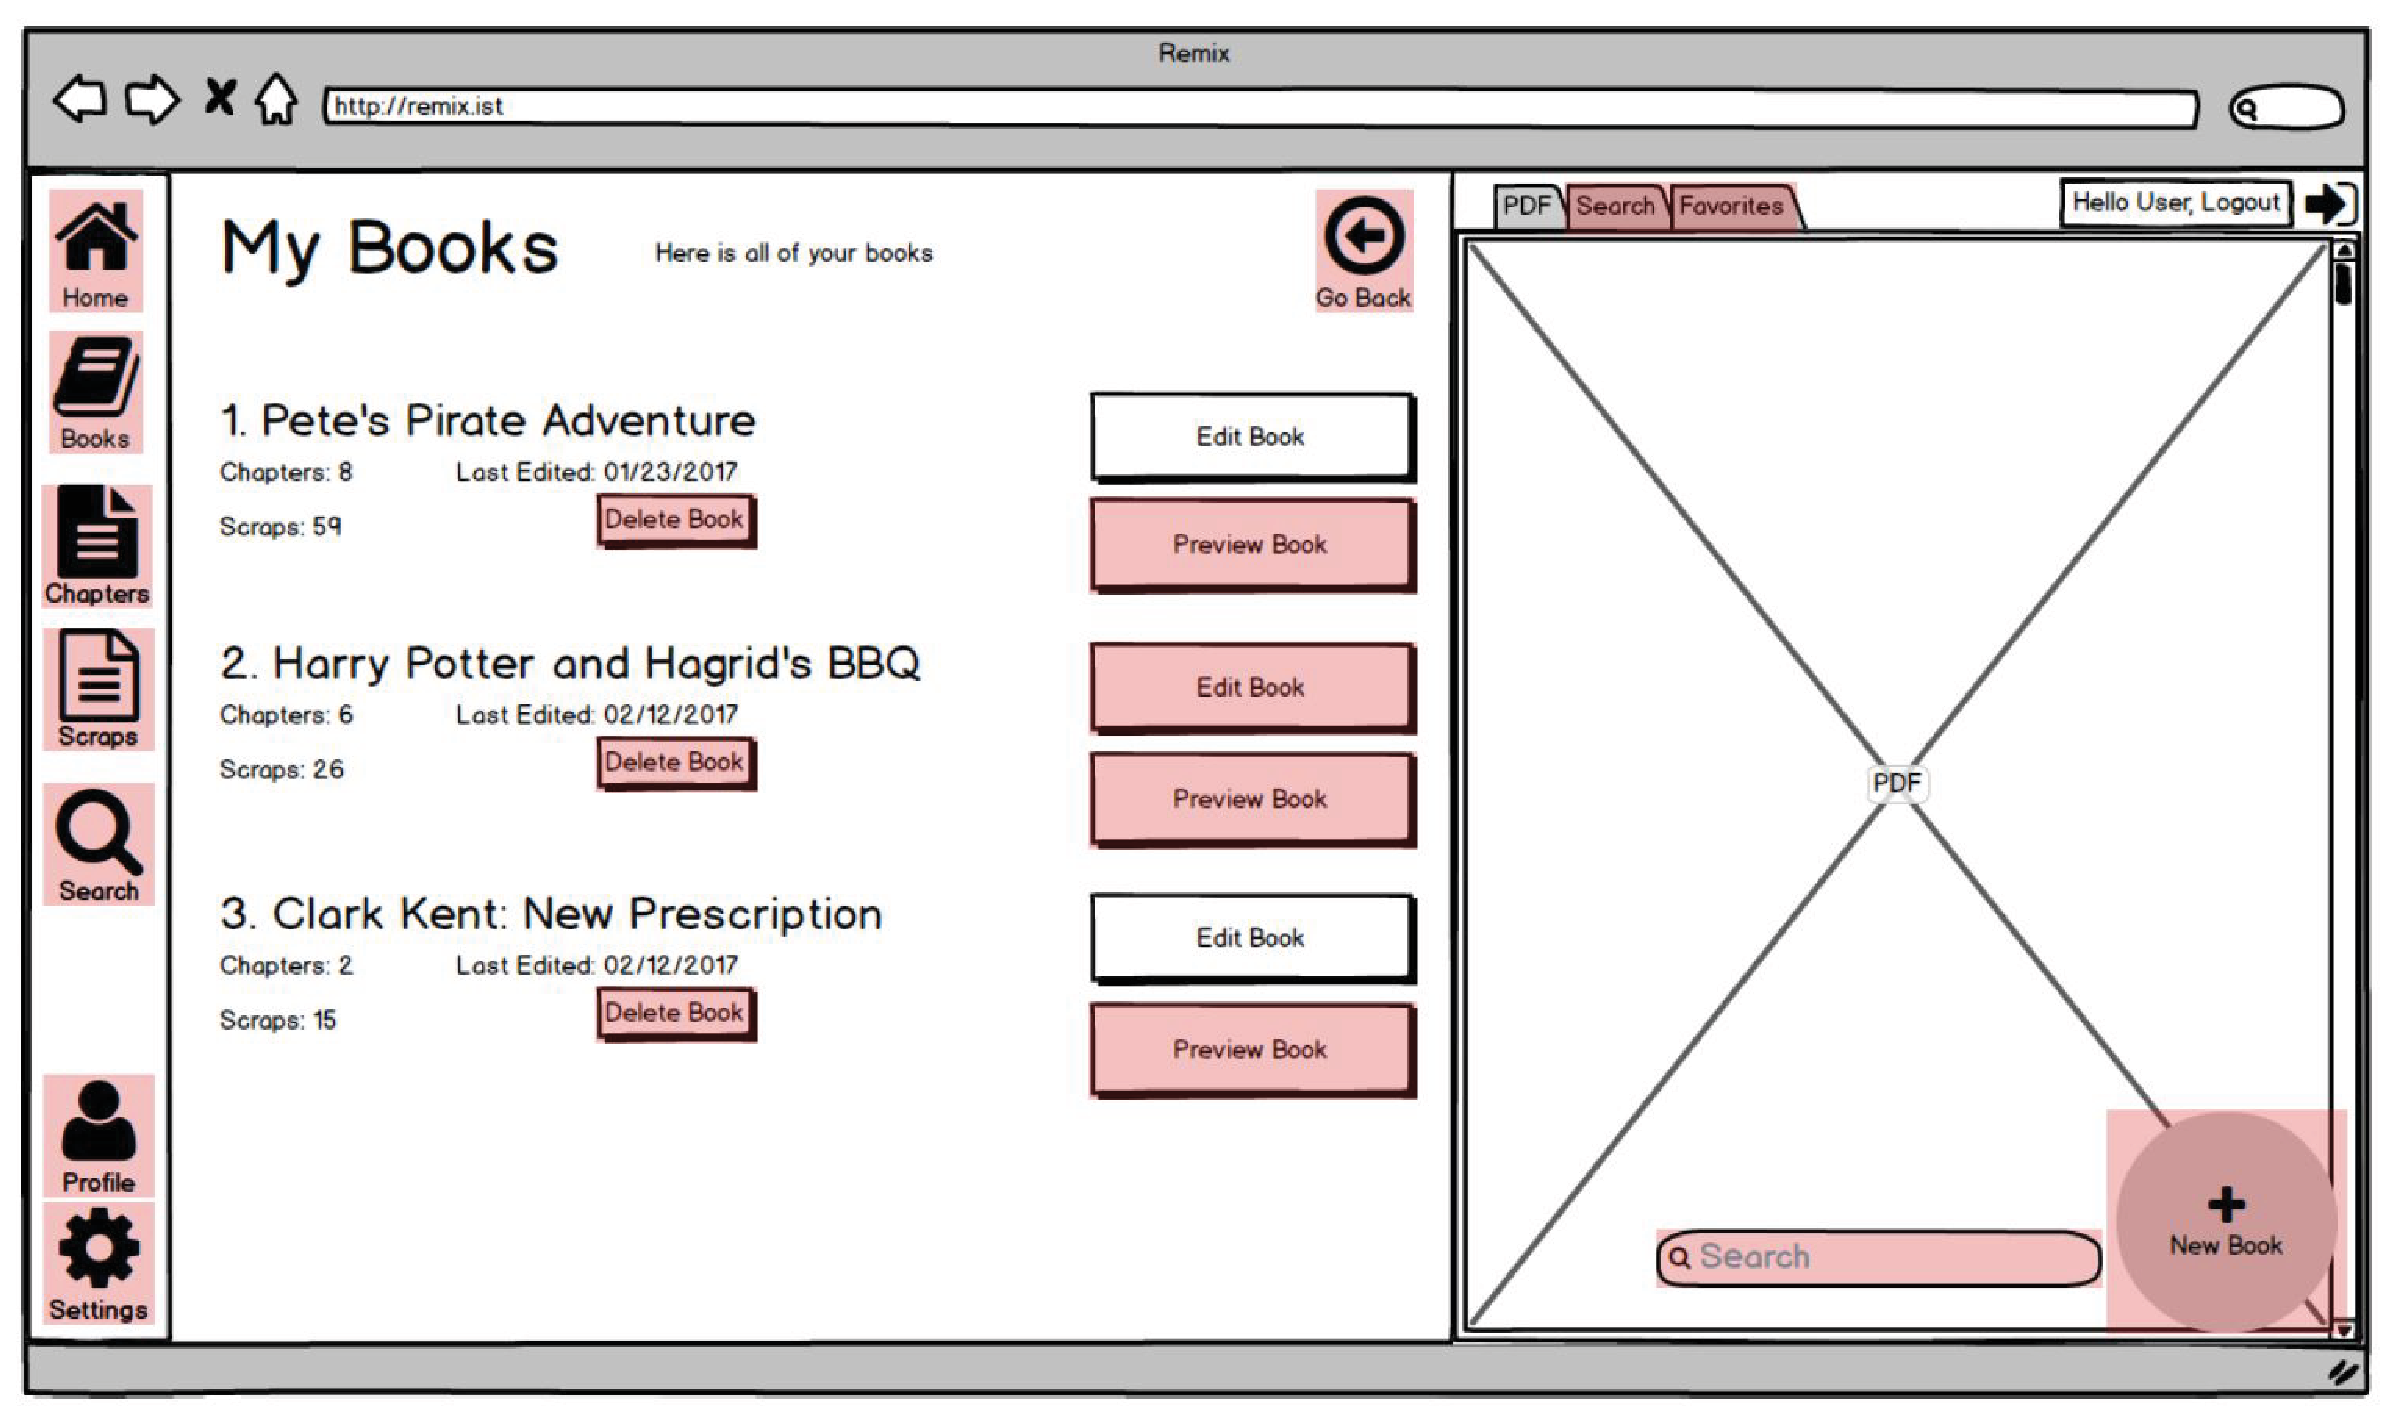
\includegraphics[width=\textwidth]{images/balsamiq}
		\caption{Here is one medium fidelity prototype, created in balsamiq, that allowed for users to provide feedback about the basic ideas of placement without worrying about finalized plans.}
	\end{figure}
	
	\begin{figure}[ht!]
		\centering
		
\includegraphics[width=\textwidth]{images/pdfpreview}
		\caption{Here is one high fidelity prototype. This was created using basic web HTML and our Aurelia framework and the use of a hard coded PDF to display a document. This was used as a learning exercise.}
	\end{figure}
	
	\begin{figure}[ht!]
		\centering
		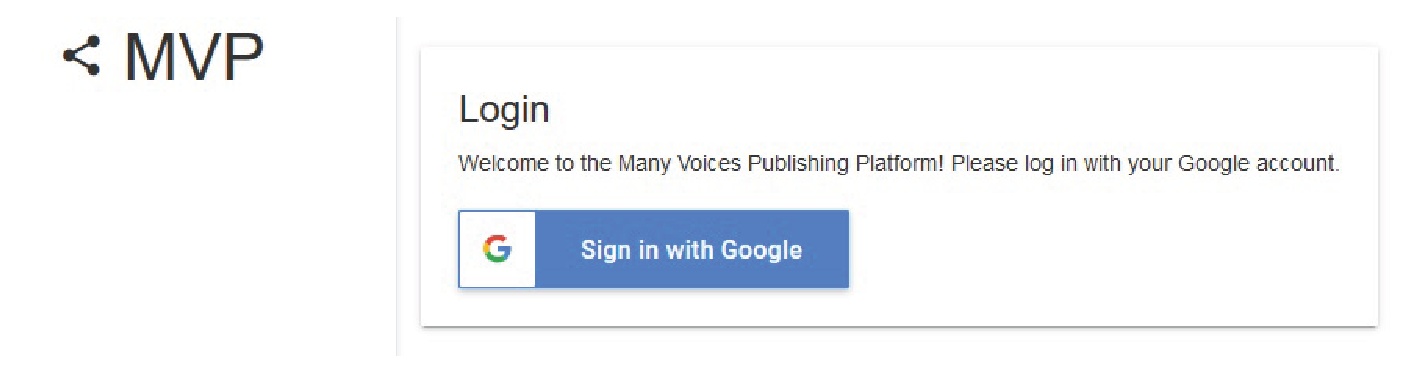
\includegraphics[width=\textwidth]{images/login_page}
		\caption{Here is the final product login page, which uses Google OAuth to abstract our need for security.}
	\end{figure}
	
	\begin{figure}[ht!]
		\centering
		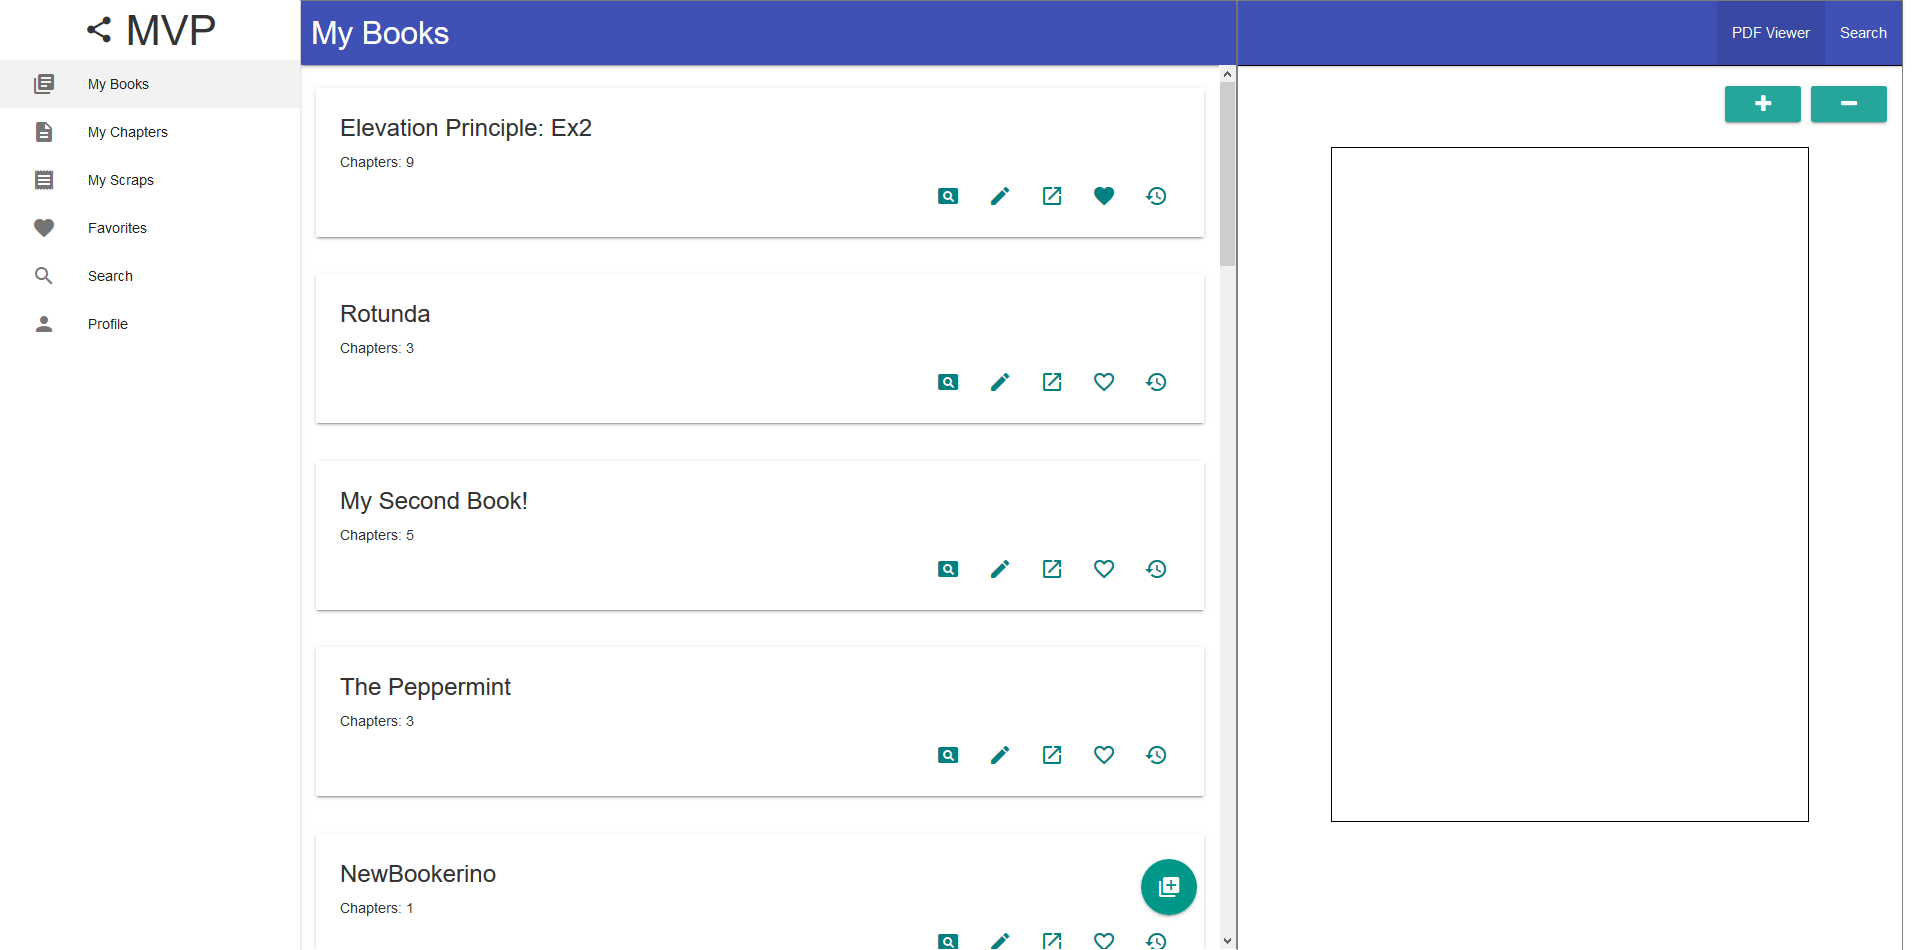
\includegraphics[width=\textwidth]{images/mybooks}
		\caption{Here is the final product my books page, showing sample textbook data.}
	\end{figure}
	
	\begin{figure}[ht!]
		\centering
		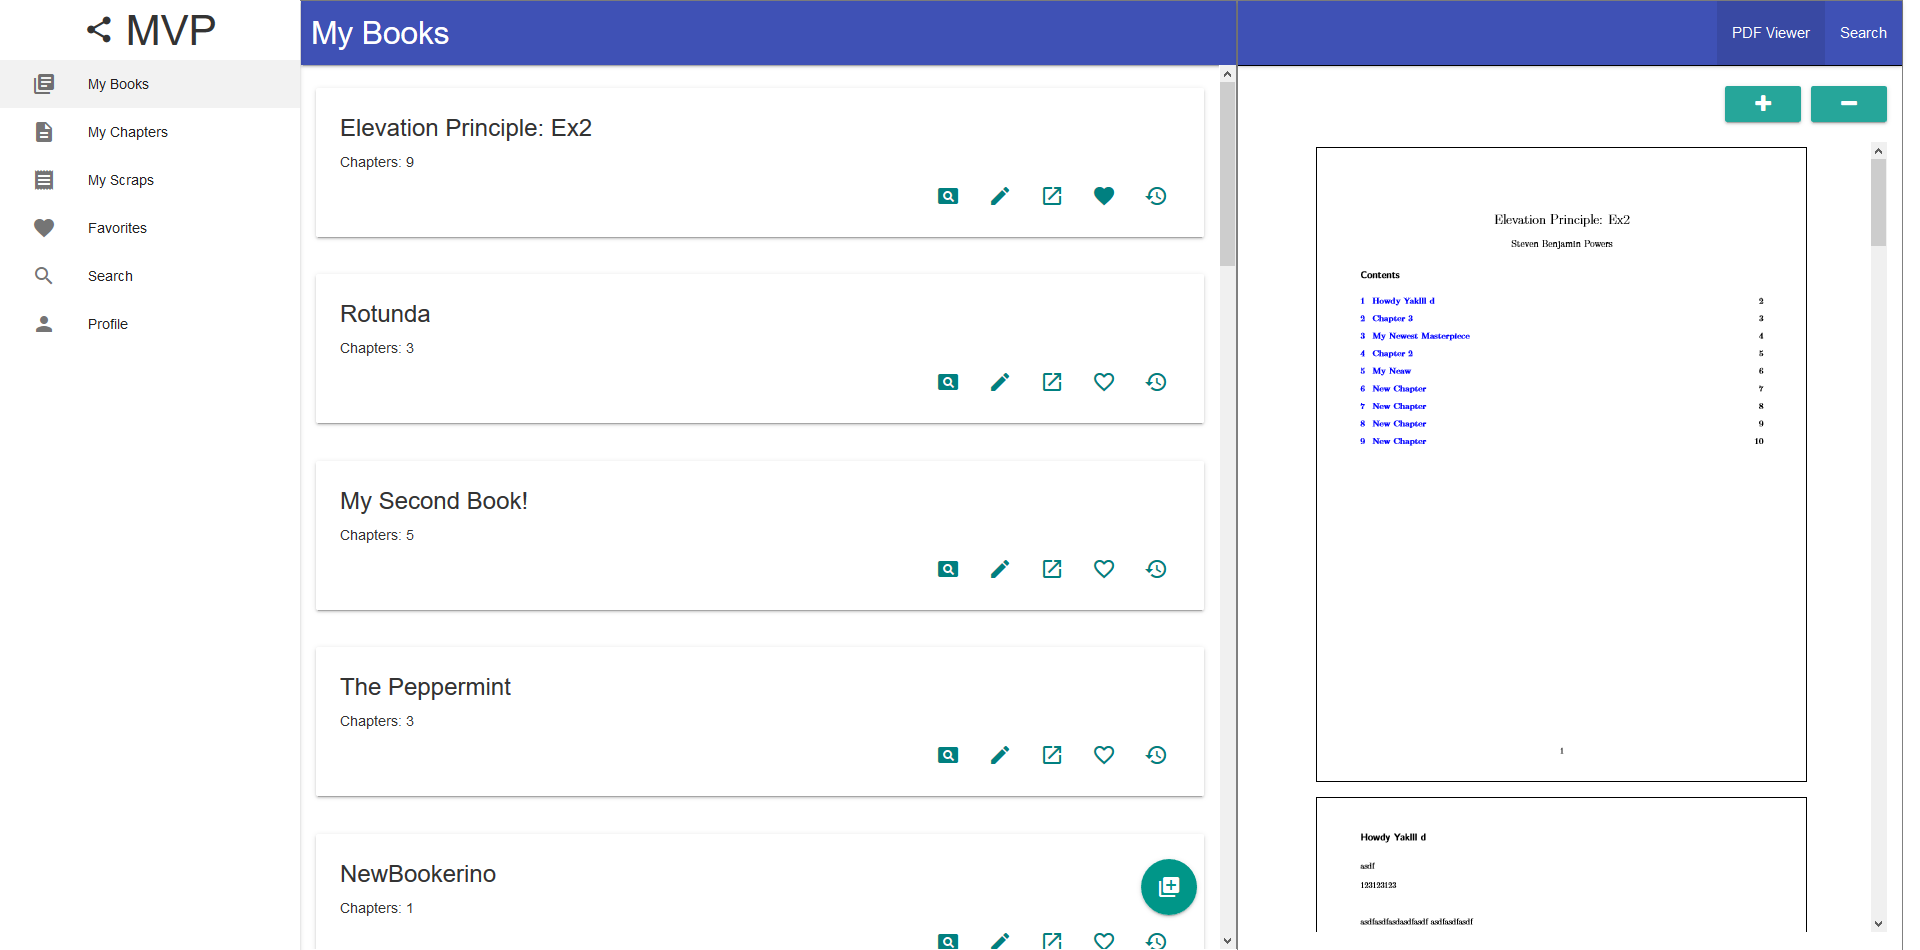
\includegraphics[width=\textwidth]{images/mybooks_preview}
		\caption{Here is the final product my books page, previewing a textbook.}
	\end{figure}
	
	\begin{figure}[ht!]
		\centering
		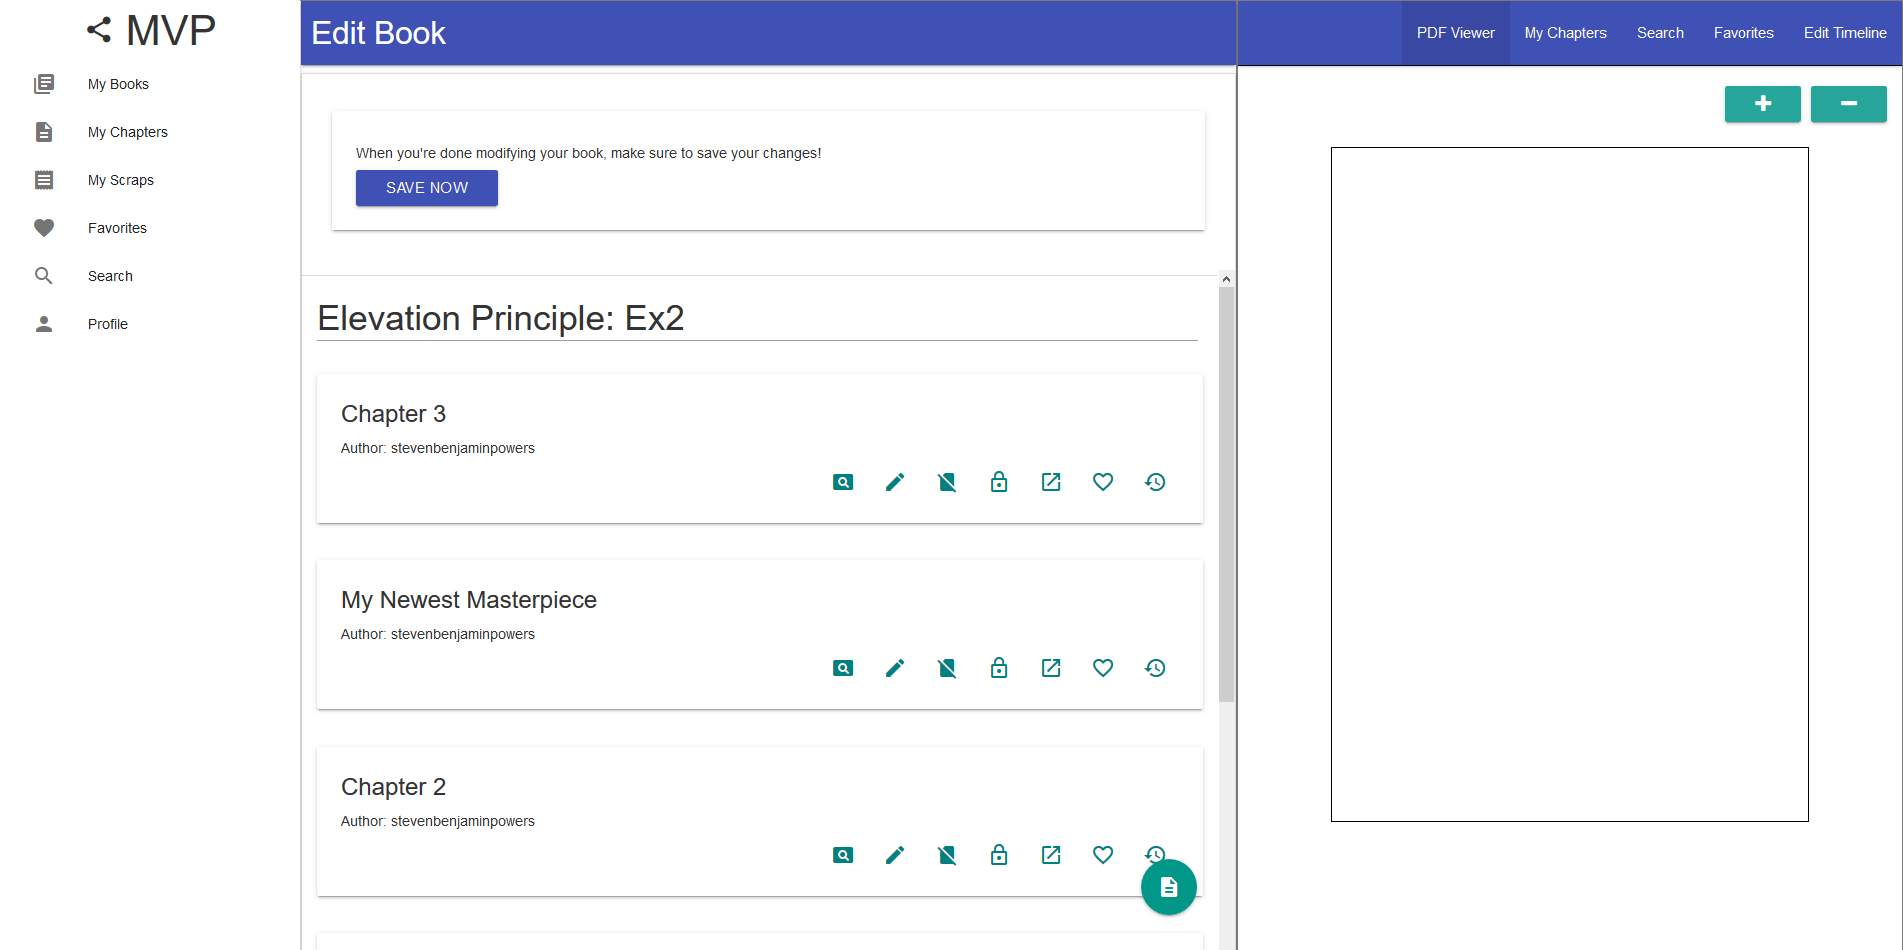
\includegraphics[width=\textwidth]{images/editbook}
		\caption{Here is the final product edit books page, allowing the user to edit chapters within a book.}
	\end{figure}
	
	\begin{figure}[ht!]
		\centering
		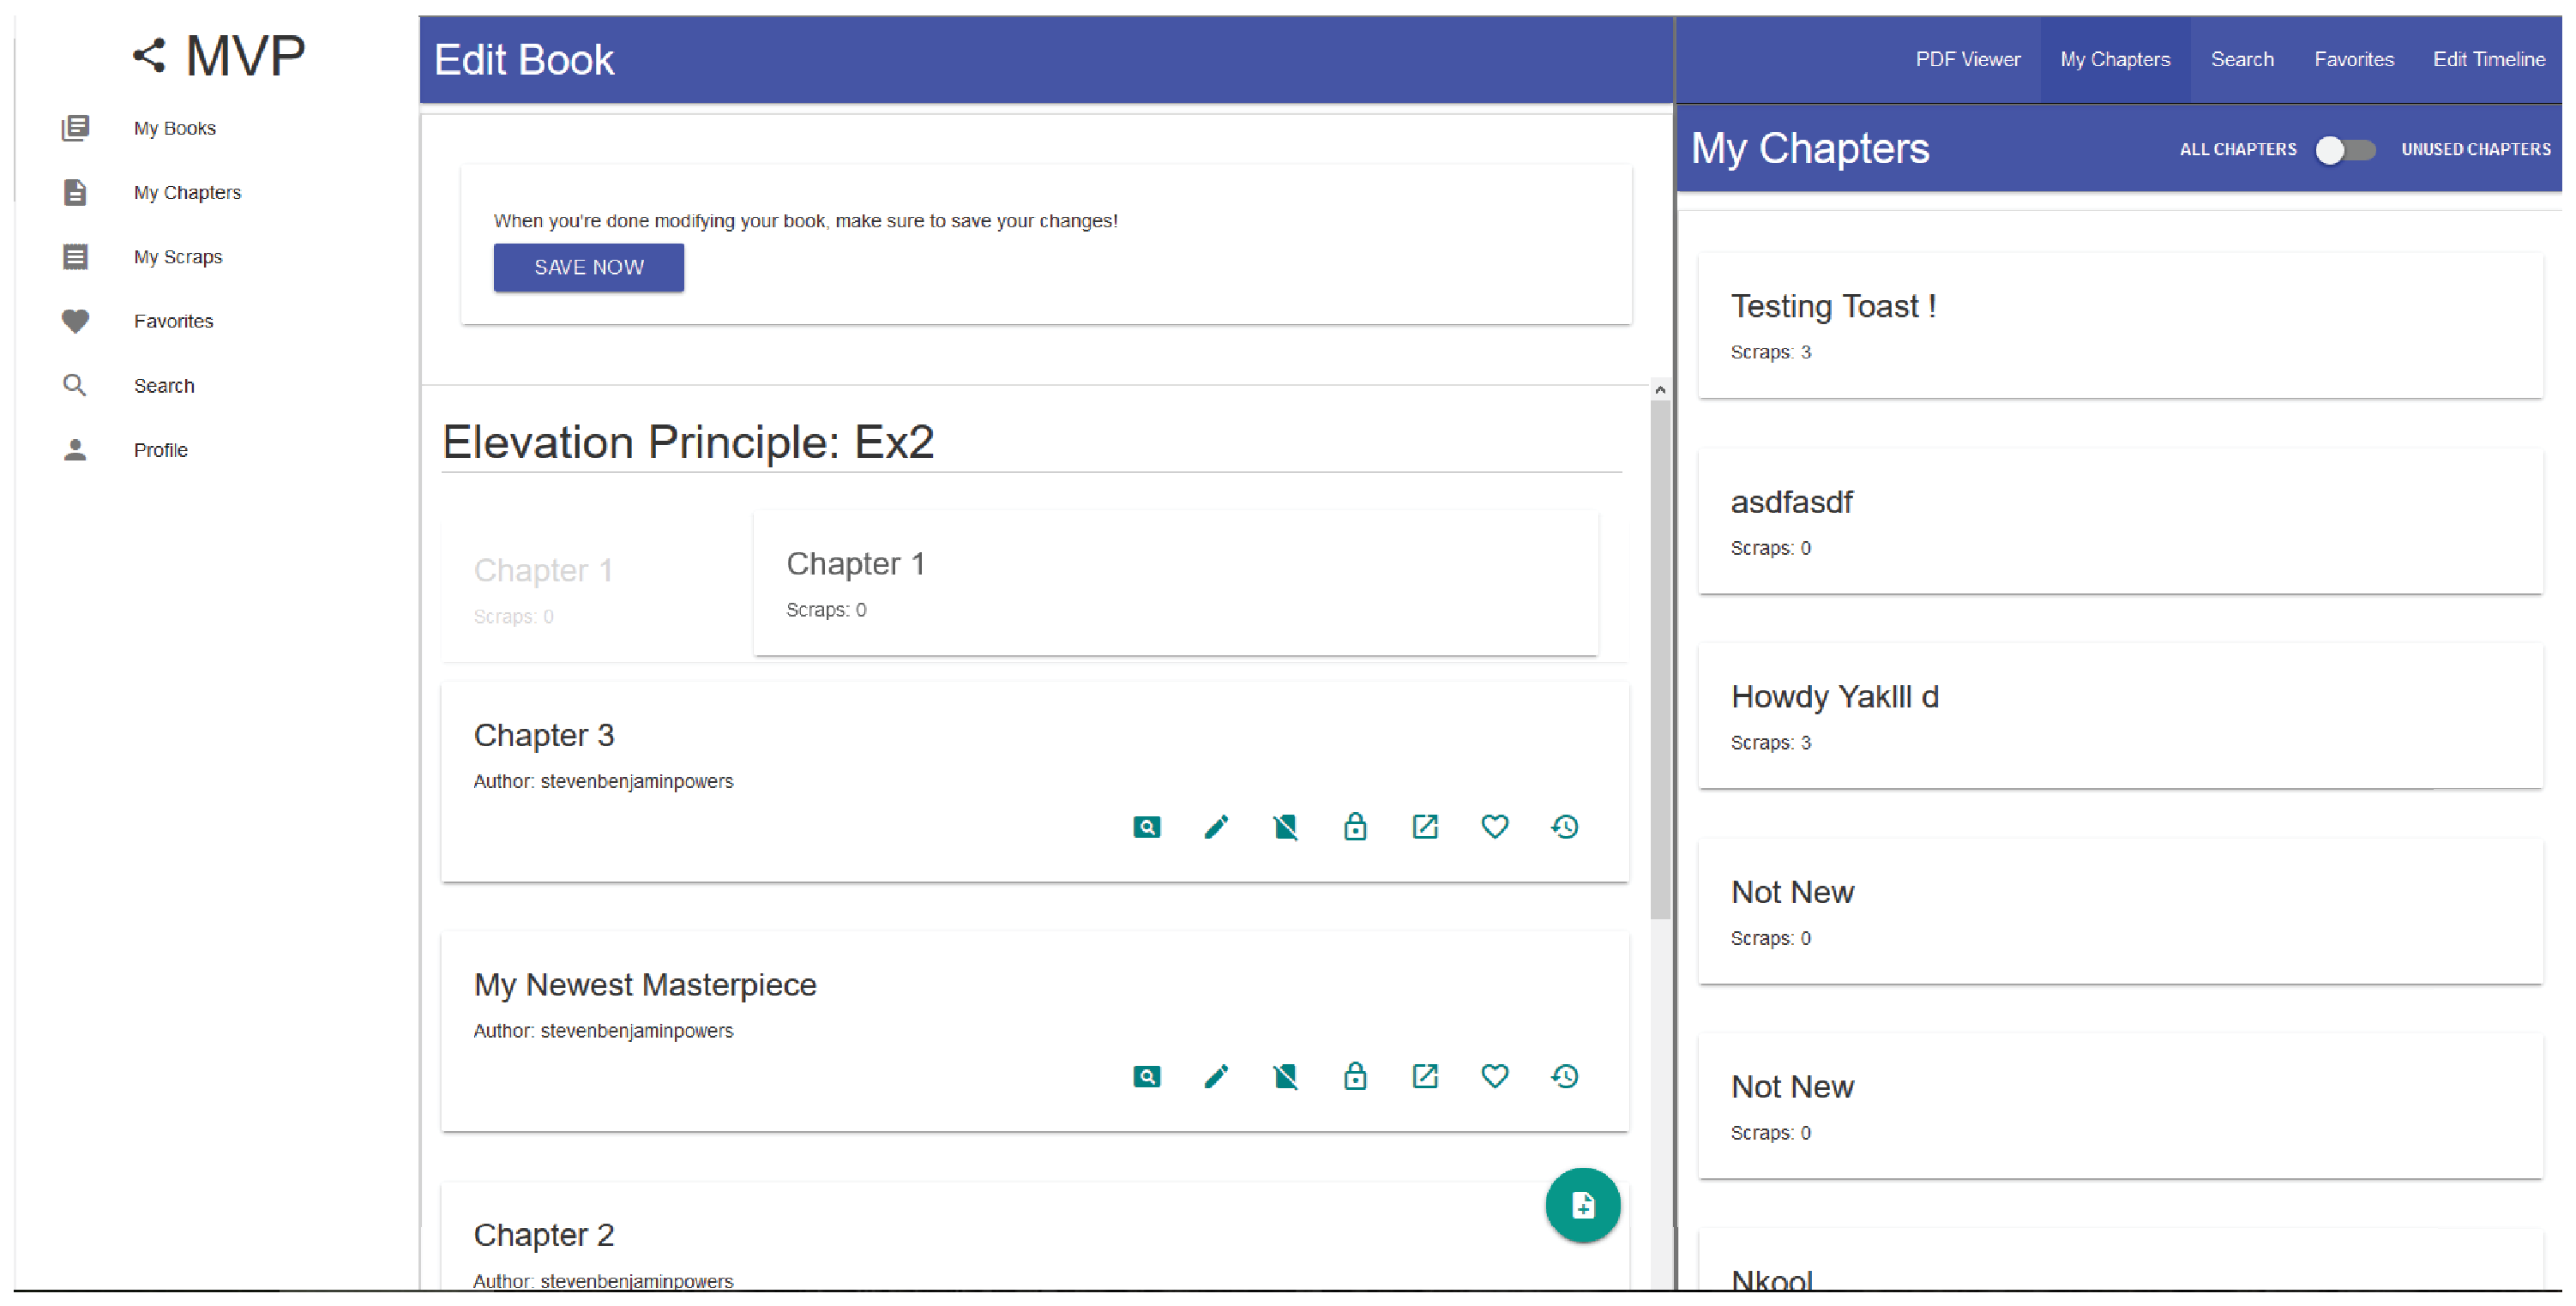
\includegraphics[width=\textwidth]{images/editbook_drag}
		\caption{Here is the final product edit books page, showing the use of drag and drop from a user's chapters.}
	\end{figure}
	
	\begin{figure}[ht!]
		\centering
		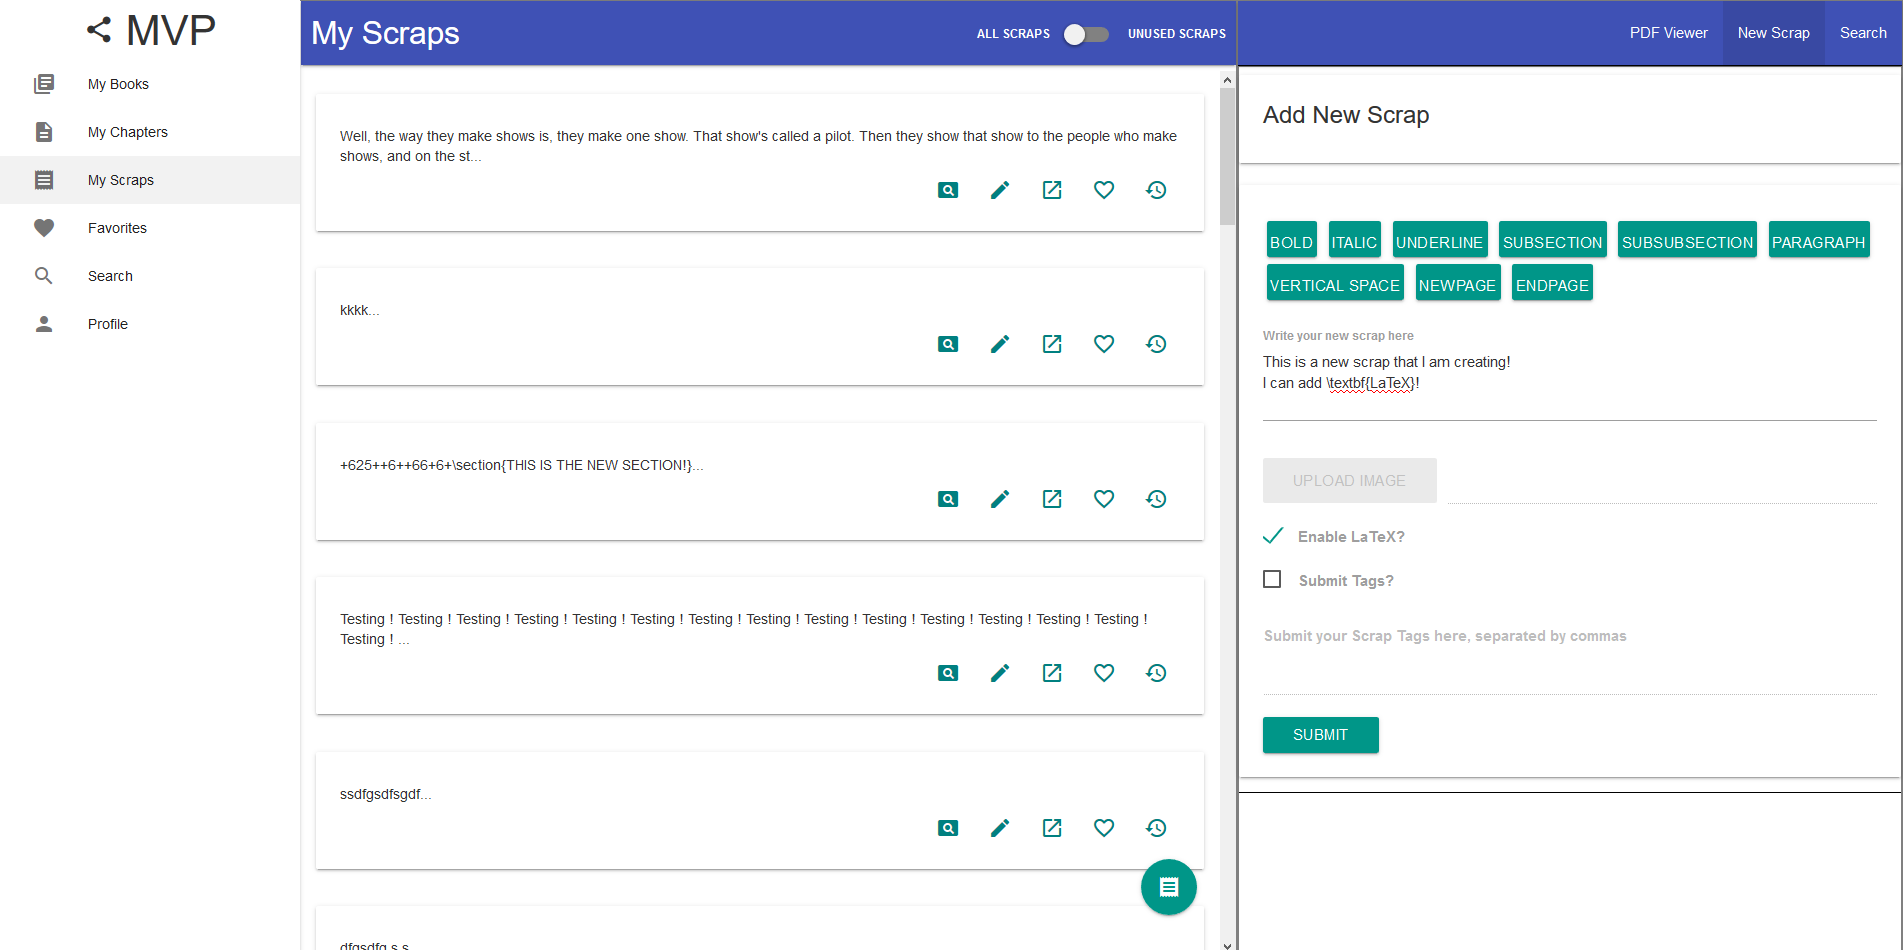
\includegraphics[width=\textwidth]{images/newscrap}
		\caption{Here is the final product new scrap page, showing how easy it is for a user to create a new scrap and even enable more advanced features by using LaTeX..}
	\end{figure}


\end{document}
